\documentclass[11pt, a4paper, norsk]{NTNUoving}
\usepackage[utf8]{inputenc}
\usepackage[T1]{fontenc}
\usepackage{tikz}
\usepackage{ifthen}
\usepackage{tikz-3dplot}
\usepackage{tikzsymbols}


\ovingnr{3}    % Nummer på innlevering
\semester{Våren 2020}
\fag{TMA 4105} %4105 er matte 2, 4115 er matte 3
\institutt{Institutt for matematiske fag}

\newenvironment{matrise}[1][]{
        \left[
            \begin{array}{#1}
    }
    {    
    \end{array}
    \right]           
}

\newenvironment{indreprod}{
    \langle
}{
\rangle}

\newcommand{\R}{\mathbb{R}}
\renewcommand{\P}{\mathcal{P}}

\begin{document}
%#################################################
%Dette er for enkel copy-pasting
\ifx
%-------------------------
\begin{oppgave}
    \begin{punkt}
        \begin{align*}
        
        
        \end{align*}
    \end{punkt}
\end{oppgave}
%-------------------------
\begin{tikzpicture}
        \draw[step=1cm,gray,very thin] (-5.9,-5.9) grid (5.9,5.9);
        \draw (-6,0) -- (6,0);
        \draw (0,-6) -- (0,6);
        \draw[->] (-6,0) -- (6,0); 
        \draw[->] (0,-6) -- (0,6);
        \draw (0, 6.2) node {y};
        \draw (6.2, 0) node {x};
\end{tikzpicture}
\fi

%Her begynner dokumentet
%#####################################
\begin{oppgave}
    Her virker sylinderkoordinater fornuftig. Da får vi $0 < \sqrt{r^2+z^2} < 1-|z|$, og $\delta(x, y, z) =(r^2+z^2)^{-\frac{3}{4}}$. Videre har vi da at $0 < r^2 < z^2+1-2|z|-z^2$. For $z>0$ gir det
    \begin{align*}
        &0< -2z+1\\
        &z<\frac{1}{2},
    \end{align*}
    
    og for negativ $z$
    \begin{align*}
        &0< 2z+1\\
        &z > -\frac{1}{2}.
    \end{align*}
    
    For å finne massen må vi finne $\int\int\int\delta(x, y, z)dV$. Av symmetrigrunner blir det
    \begin{align*}
        2\int_0^{2\pi}\int_0^{\frac{1}{2}}\int_0^{\sqrt{1-2z}}(r^2+z^2)^{-\frac{3}{4}}rdrdzd\theta&=\int_0^{2\pi}\int_0^{\frac{1}{2}}\int_{z^2}^{(z-1)^2}(u)^{-\frac{3}{4}}dudzd\theta
        \\&=8\pi\int_0^{\frac{1}{2}}[u^{\frac{1}{4}}]_{z^2}^{(z-1)^2}dz
        \\&=8\pi\int_0^\frac{1}{2}\sqrt{|z-1|}-\sqrt{z}dz
        \\&=8\pi \int_{0}^{\frac{1}{2}}\sqrt{1-z}-\sqrt{z}dz
        \\&=8\pi \left(-\int_{1}^{\frac{1}{2}}\sqrt{u}du-\int_0^{\frac{1}{2}}\sqrt{z}dz\right)
        \\&=-\frac{16\pi}{3}\left( [u^\frac{3}{2}]_{1}^{\frac{1}{2}}+[z^\frac{3}{2}]_{0}^{\frac{1}{2}}\right)
        \\&=-\frac{16\pi}{3}\left(\frac{1}{2\sqrt{2}}-1+\frac{1}{2\sqrt{2}}-0\right)
        \\&=-\frac{16\pi}{3}\left(\frac{\sqrt{2}}{2}-1\right)
        \\&=\frac{16\pi}{3}\left(\frac{2-\sqrt{2}}{2}\right)
        \\&=\frac{16\pi-8\sqrt{2}\pi}{3}
    \end{align*}
\end{oppgave}

\begin{oppgave}
Her ser vi at i $yz$-planet($x=0$, $r=y$) får vi en sirkel med radius 1, med senter i $y=2$. Å rotere det $2\pi$ om $z$-aksen gir en torus. Se figur \ref{fig:my_label}
\begin{figure}
    \centering
    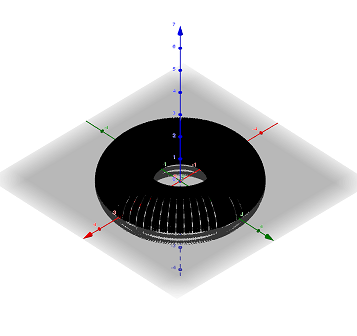
\includegraphics{fig.png}
    \caption{Likningen i oppgave 2 ga en torus med indre radius 1 og ytre radius 3.}
    \label{fig:my_label}
\end{figure}

Volumet finner man ved å ta trippeltingegralet av $1$. Grensene for $\theta$ er $0$ og $2\pi$, for $z$ er de $\pm 1$, mens for $r$ må vi løse likningen med hensyn på $r$. 
\begin{align*}
    (r-2)^2+z^2 &\leq 1\\
    (r-2)^2 &\leq 1-z^2\\
    -\sqrt{1-z^2} \leq r&-2 \leq \sqrt{1-z^2}\\
    -\sqrt{1-z^2}+2 \leq r& \leq \sqrt{1-z^2}+2
\end{align*}
Vi får da at volumet er lik
\begin{align*}
    \int_0^{2\pi}\int_{-1}^1\int_{-\sqrt{1-z^2}+2}^{\sqrt{1-z^2}+2}rdrdzd\theta&=\pi\int_{-1}^1\left[r^2\right]_{-\sqrt{1-z^2}+2}^{\sqrt{1-z^2}+2}dz
    \\&=\pi\int_{-1}^{1}1-z^2+4\sqrt{1-z^2}+4-(1-z^2-4\sqrt{1-z^2}+4)dz
    \\&=\pi\int_{-1}^{1}8\sqrt{1-z^2}dz.
\end{align*}
Med substitusjonen $z=\sin\left(\Laughey[1.4]\right), dz=\cos\left(\Laughey[1.4]\right)d\, \Laughey[1.4],$ får vi
\begin{align*}
    8\pi\int_{-1}^{1}\sqrt{1-z^2}dz&=8\pi \int_{-\frac{\pi}{2}}^{\frac{\pi}{2}}\cos^2 \left(\Laughey[1.4]\right) d\, \Laughey[1.4]
    \\&=4\pi\int_{-\frac{\pi}{2}}^{\frac{\pi}{2}}\cos \left(2\, \Laughey[1.4]\right) +1d\, \Laughey[1.4]
    \\&=4\pi \left[\frac{1}{2}\sin \left(2\, \Laughey[1.4]\right) + \Laughey[1.4] \right]_{-\frac{\pi}{2}}^{\frac{\pi}{2}}
    \\&=4\pi\left(2\frac{\pi}{2}\right)
    \\&=4\pi^2
\end{align*}
\end{oppgave}
\begin{oppgave}
    Dersom $\frac{\partial}{\partial z}2xy+z^2\neq\frac{\partial}{\partial y}2ayz$ er ikke feltet konservativt. Det gir at $a$ må være lik 1. Det er ikke dermed gitt at feltet er konservativt, men $a$ kan ikke være ulik 1. 
    
    For å finne en potensialfunksjon kan man ta integralet av hver komponent med hensyn på den komponenten:
\begin{align*}
    &\int 1+y^2dx = x+y^2x+C
    \\&\int 2xy+z^2dz = xy^2+yz^2+C
    \\&\int 2yzdz = yz^2+C
\end{align*}
Her ser vi at $\phi(x, y, z)=x+y^2x+yz^2$ er en løsning. Siden potensialfunksjonen eksisterer er vektorfeltet konservativt, og dermed er integralet lik differansen mellom endepunktene til potensialfunksjonen. Altså
\begin{align*}
    &\phi(t, \sin\pi t, \cos\pi t)=t+t\sin^2\pi t+\sin\pi t*\cos^2 \pi t\\
    &t=0: 0+0^2+1*0=0\\
    &t=\frac{1}{2}: \frac{1}{2}+\frac{1}{2}1^2+1*0^2=1\\
    &\int_\mathcal{C}\textbf{F}_a\cdot d\textbf{r}=1-0=1
\end{align*}
\end{oppgave}
\begin{oppgave}
    \begin{align*}
        x^2+y^2+z^2&=3\\
        2z+z^2&\leq3\\
        -3 \leq z& \leq 1
    \end{align*}
    Likningen for paraboloiden tilsier at $z\geq 0$. Med polarkoordinater får vi $2z=r^2$, som gir at projeksjonen av $S$ ned i $xy$-planet er $r^2\leq 2*1$, altså $x^2+y^2\leq 2$.
    
    Arealet av $S$ er gitt ved $\int\int_SdS$. Grensene for $x$ og $y$ er gitt ved $1=\frac{1}{2}(x^2+y^2)$.
    \begin{align*}
        \int\int_SdS&=\int_{-\sqrt{2}}^{\sqrt{2}}\int_{-\sqrt{2-x^2}}^{\sqrt{2-x^2}}\sqrt{\left(\frac{\partial f}{\partial x}\right)^2+\left(\frac{\partial f}{\partial y}\right)^2+1}dydx
        \\&=\int_{-\sqrt{2}}^{\sqrt{2}}\int_{-\sqrt{2-x^2}}^{\sqrt{2-x^2}}\sqrt{x^2+y^2+1}dydx
    \end{align*}
    Dette er et vanskelig integral. Det er enklere å løse med polarkoordinater. Det gir
    \begin{align*}
        \int_{-\sqrt{2}}^{\sqrt{2}}\int_{-\sqrt{2-x^2}}^{\sqrt{2-x^2}}\sqrt{x^2+y^2+1}dydx&=\int_0^{2\pi}\int_0^{\sqrt{2}}\sqrt{r^2+1}rdrd\theta
        \\&=2\pi\int_0^{\sqrt{2}}\sqrt{r^2+1}rdr
        \\&=\pi\int_1^3\sqrt{u}du
        \\&=\pi\frac{2}{3}\left[u^\frac{3}{2}\right]_1^3
        \\&=\frac{2\pi}{3}(3\sqrt{3}-1)
    \end{align*}
\end{oppgave}
\end{document}
